\documentclass[10pt,a4paper]{article}
\usepackage[a4paper,landscape,margin=14mm]{geometry}
\usepackage{fontspec}
\setmainfont{Helvetica}
\usepackage{longtable,booktabs,array,ragged2e}
\usepackage{xcolor}
\usepackage{graphicx}
\usepackage{titlesec}
\usepackage[hidelinks]{hyperref}
\usepackage{enumitem}
\usepackage{fancyhdr}

\definecolor{accent}{HTML}{1B4F72}
\definecolor{warn}{HTML}{922B21}
\definecolor{soft}{HTML}{F4F6F7}

\titleformat{\section}{\Large\bfseries\color{accent}}{\thesection.}{0.5em}{}
\titleformat{\subsection}{\large\bfseries\color{accent!80!black}}{\thesubsection.}{0.5em}{}
\setlist{nosep,leftmargin=*}

\pagestyle{fancy}\fancyhf{}
\renewcommand{\headrulewidth}{0.4pt}
\lhead{\small\color{accent}PhishDriftBench + DASH}
\rhead{\small\color{accent}\thepage}

\newcolumntype{L}[1]{>{\RaggedRight\arraybackslash}p{#1}}

\begin{document}

%================== TITLE ==================
\begin{center}
{\LARGE\bfseries\color{accent} PhishDriftBench + DASH}\\[4mm]
{\large The Reported--Deployed Gap in Phishing URL Detection:\\
A Time-, Source-, Provenance- and Evasion-Aware Benchmark\\
with Drift-Aware Selective Hardening}\\[3mm]
{\small Final Year Project --- Project Definition, Literature Review and Architecture}
\end{center}
\vspace{3mm}

%================== ABSTRACT ==================
\section{Abstract}

Published phishing URL detectors routinely report 97--99.5\% accuracy, yet these figures are
almost always produced under one evaluation protocol: a random or $k$-fold split of a single
dataset, balanced at roughly 50\% phishing prevalence, with no adversary in the loop. Each of
those choices is individually defensible and collectively misleading. Random splits leak time,
because phishing URLs arrive in campaigns whose near-identical members land in both train and
test partitions. Single-source evaluation hides source-specific artifacts --- a feature can carry
\emph{opposite} meaning in different corpora. Balanced test sets conceal the base-rate problem: a
detector with 99\% accuracy and a 1\% false-positive rate, deployed at a real prevalence of
$1{:}10^{4}$, yields precision near 1\%.

This project builds \textbf{PhishDriftBench}, a four-axis evaluation protocol that measures
detectors across time, across data sources, against rule-based and generative evasion, and at
deployment-realistic class priors. Under this protocol we re-evaluate five representative
architectures drawn from the base papers. We add a \textbf{feature-provenance audit} that
separates statically computable lexical features from those requiring a live network lookup, and
quantifies how much reported accuracy is attributable to lookup artifacts rather than phishing
semantics. Finally we propose \textbf{DASH} (Drift-Aware Selective Hardening), a lightweight
mitigation combining drift-stability feature weighting, unsupervised drift detection, a bounded
active-labelling budget, and a calibrated abstention band. The project is \textbf{URL-only}: no
page is fetched, rendered, hosted or transmitted at any point.

\vspace{2mm}
\noindent\fcolorbox{warn}{warn!5}{%
\begin{minipage}{\dimexpr\textwidth-2\fboxsep-2\fboxrule}
\textbf{\color{warn}Status:} design and protocol complete; experiments not yet run. Every
quantitative claim in the accompanying paper draft is an explicit unfilled placeholder. No
results are reported until they are measured.
\end{minipage}}

%================== IMPROVEMENTS ==================
\section{Improvements over the base papers}

Each improvement names a specific, verified gap in the ten base papers.

\begin{enumerate}[label=\textbf{\arabic*.}]

\item \textbf{Temporal evaluation instead of random splits.}
\emph{Gap:} 0 of 10 base papers uses a chronological split.
\emph{Improvement:} train on URLs first observed $\le T$, test on disjoint windows at $+1$, $+3$,
$+6$ and $+12$ months; report a \textbf{decay curve}, not a single accuracy. Paper~5 accidentally
demonstrates why --- 99.35\% on its 2025 data but 89.17\% on an older corpus.

\item \textbf{True cross-source transfer.}
\emph{Gap:} only 1 of 10 (X-PHIDE) performs genuine transfer; Paper~5 evaluates on multiple
datasets but \textbf{retrains per dataset}, which measures dataset difficulty, not transfer.
\emph{Improvement:} train once, evaluate on all source pairs plus leave-one-source-out.

\item \textbf{Prevalence-corrected reporting.}
\emph{Gap:} 0 of 10 reports precision at a realistic deployment base rate.
\emph{Improvement:} report precision, FPR and alerts per $10^{6}$ URLs at prevalences of
$1{:}10^{2}$, $1{:}10^{3}$ and $1{:}10^{4}$, alongside balanced figures for comparability.

\item \textbf{Evasion testing against our own detector.}
\emph{Gap:} Paper~10 catalogues cloaking thoroughly; \textbf{no method paper evaluates its own
detector against that catalogue.} Paper~4 states outright that homograph attacks were never
systematically evaluated.
\emph{Improvement:} \textbf{E1} label-preserving transformations from the cloaking taxonomy
(homoglyph/IDN substitution, subdomain and path padding, percent-encoding, shortener wrapping,
TLD swap, hyphenated brand insertion) and \textbf{E2} URLs from a contemporary generative model.

\item \textbf{Feature-provenance and lookup-dependency audit} \emph{(most novel)}.
\emph{Gap:} no base paper --- and no adjacent work we could find --- asks \emph{where} a feature's
value comes from or \emph{when} it was resolved.
\emph{Improvement:} classify every feature as \textbf{P1} static-lexical, \textbf{P2}
lookup-at-inference (WHOIS, DNS, SSL, domain age, shortener expansion) or \textbf{P3} third-party
reputation; then measure accuracy with P2/P3 ablated, accuracy when P2 features are resolved
\emph{today} versus at collection time, and recall when the lookup channel is unavailable or
attacker-controlled. The hazard is concrete: Paper~6 reports WHOIS, DNS and domain-age features
over a 549,346-URL corpus containing \textbf{only URL strings}. If those lookups were performed
retrospectively they encode \emph{domain mortality} --- phishing domains die within days,
legitimate ones persist for years --- which any classifier can exploit without learning anything
about phishing. Paper~4, which deliberately avoids third-party features, is the control.

\item \textbf{Drift-stability feature scoring.}
\emph{Gap:} drift is \emph{named} by 4 of 10 papers and \emph{implemented} by none.
\emph{Improvement:} score each feature by Population Stability Index across time windows and
sources plus the variance of its permutation importance; partition into drift-stable and
drift-brittle \emph{before} deployment. Validation target: the HTTPS inversion X-PHIDE found
(100\% of legitimate URLs in PhiUSIIL, 59.2\% in their own corpus) should be flagged without
access to the second corpus's labels.

\item \textbf{DASH --- a mitigation, not just a diagnosis.}
\emph{Gap:} 0 of 10 proposes any drift mitigation.
\emph{Improvement:} (i) stability-weighted training; (ii) \textbf{unsupervised} drift detection
over the prediction-confidence stream, requiring no labels --- the binding constraint in
deployment; (iii) a bounded active-labelling budget ($\approx 2\%$ of the window by uncertainty
sampling) on drift alarm; (iv) a calibrated abstention band that escalates instead of guessing,
reported as a coverage--risk curve.

\item \textbf{Duplicate-leakage probe (supporting).}
Report exact and near-duplicate rates across the train/test boundary for every corpus, and
accuracy before and after deduplication. With $k$-fold CV over scraped corpora, campaign
duplicates are near-certain.

\end{enumerate}

\clearpage
%================== ARCHITECTURE ==================
\section{System architecture}

\begin{center}
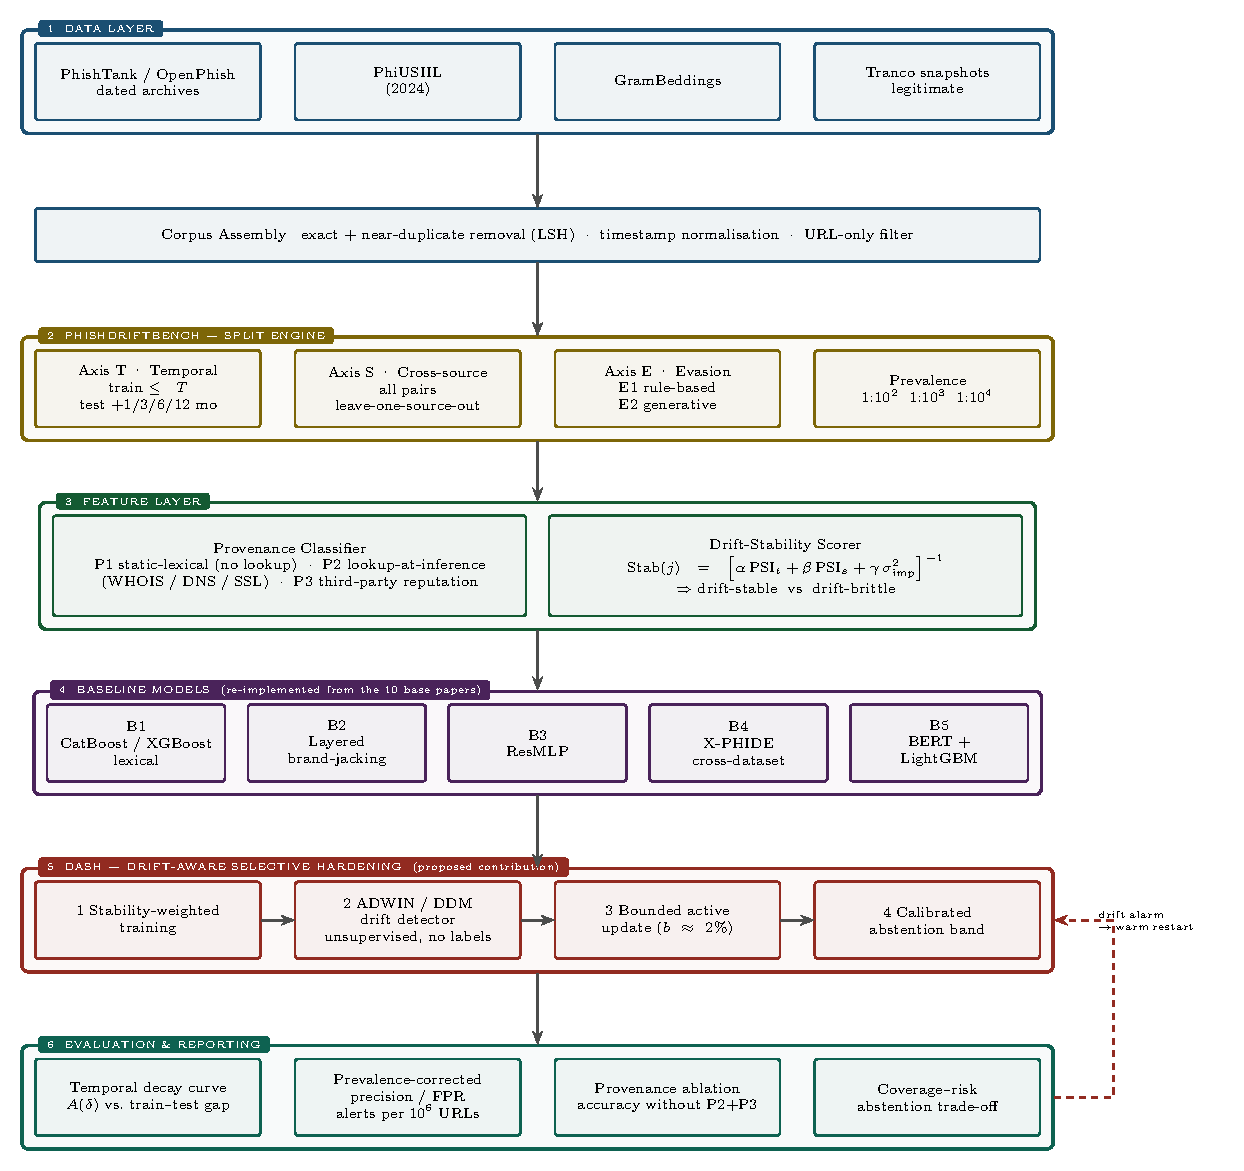
\includegraphics[height=0.74\textheight,keepaspectratio]{arch.pdf}
\end{center}

\vspace{1mm}
\noindent\small The pipeline is strictly URL-only. Layer~1 assembles dated corpora; Layer~2
generates the four evaluation axes; Layer~3 classifies features by provenance and scores their
drift stability; Layer~4 hosts five baselines re-implemented from the base papers; Layer~5 is the
proposed DASH mitigation; Layer~6 produces deployment-honest reporting. The dashed return path
carries a drift alarm back into DASH for a warm restart.

\clearpage
%================== LITERATURE REVIEW ==================
\section{Literature review}

Ten base papers, all published 2023 or later: eight method or empirical studies plus two reviews.

\vspace{2mm}
{\scriptsize
\setlength{\tabcolsep}{3pt}
\renewcommand{\arraystretch}{1.15}
\begin{longtable}{@{}L{4mm} L{34mm} L{26mm} L{22mm} L{40mm} L{34mm} L{40mm} L{34mm}@{}}
\toprule
\textbf{\#} & \textbf{Title} & \textbf{Authors} & \textbf{Publication \& Year} &
\textbf{Key Findings} & \textbf{Research Gap} & \textbf{Methodology} & \textbf{Future Work}\\
\midrule
\endfirsthead
\toprule
\textbf{\#} & \textbf{Title} & \textbf{Authors} & \textbf{Publication \& Year} &
\textbf{Key Findings} & \textbf{Research Gap} & \textbf{Methodology} & \textbf{Future Work}\\
\midrule
\endhead
\bottomrule
\endfoot

1 & An Effective Detection Approach for Phishing URL Using ResMLP &
S. Remya; M. J. Pillai; K. K. Nair; S. R. Subbareddy; Y. Y. Cho &
IEEE Access, vol.~12, 2024 &
98.29\% accuracy; residual pipelining outperforms traditional ML baselines on the same features &
Blacklists cannot identify dynamic and newly registered URLs; optimal detection accuracy remains
an open pursuit &
Lexical + sentiment + domain-age features $\rightarrow$ convolutional and inverted-residual
blocks $\rightarrow$ MLP; Kaggle dataset, 80:20 random split &
Address limitations affecting practical viability; explore self-organising networks and
online-learning representations \\
\addlinespace

2 & On Phishing URL Detection Using Feature Extension &
D. He; Z. Liu; X. Lv; S. Chan; M. Guizani &
IEEE Internet of Things Journal, vol.~11, no.~24, 2024 &
Feature extension enriches information-poor URLs; two-layer BERT$\rightarrow$CNN improves
detection, including on cryptocurrency phishing &
URLs are short and carry little signal; blacklist/whitelist methods have inherent limitations &
TextRank keyword extraction builds a feature-extension library; BERT embeddings feed a CNN
classifier; single real-phishing dataset &
Extend to broader transaction-security threats in the blockchain and cryptocurrency ecosystem \\
\addlinespace

3 & Evaluating the Impact of Feature Engineering in Phishing URL Detection: A Comparative Study
of URL, HTML, and Derived Features &
Y. A. Kustiawan; K. I. Ghauth &
IEEE Access, vol.~13, 2025 &
99.45\% (CatBoost); derived features contribute most; systematic comparison across three feature
families and ten models &
Prior work studies URL \emph{or} HTML features in isolation; no comparative study of engineered
feature sets across models &
101,063-URL corpus; URL / HTML / derived feature groups $\times$ 10 ML models; single dataset,
random split &
Cascading architecture --- cheap URL analysis first, heavier content and relationship analysis
only for borderline cases; craft further derived features \\
\addlinespace

4 & PhishOFE: A Novel Machine Learning Framework for Real-Time Phishing URL Detection With
Optimized Feature Engineering &
Y. A. Kustiawan; K. I. Ghauth &
IEEE Access, vol.~13, 2025 &
99.48\% (CatBoost) with \textbf{no third-party features}, enabling real-time deployment &
Prior studies depend on outdated datasets and on third-party services that break in deployment &
Optimised feature-engineering pipeline avoiding third-party lookups; CatBoost plus comparison
models; single dataset, random split &
Homograph-attack detection via character normalisation, visual-similarity metrics and
Unicode-aware features --- explicitly \textbf{not} evaluated in the paper \\
\addlinespace

5 & Enhanced Phishing Detection Approach Using a Layered Model: Domain Squatting and URL
Obfuscation Identification and Lexical Feature-Based Classification &
R. Goenka; M. Chawla; N. Tiwari &
IEEE Access, vol.~13, 2025 &
99.35\% (XGBoost) at 12.49\,ms; but only 89.17\% on an older dataset, which the authors attribute
to 2025 target brands differing from 2018 &
Prevailing approaches overlook domain-squatting and URL obfuscation (brand-jacking), which cause
most successful phishing &
Layer~1: bad-domain features detect brand names in unwanted positions or misspelled forms;
Layer~2: lexical-feature ML classifier; own corpus + 6 datasets, \textbf{retrained per dataset} &
Extend the brand-jacking feature set beyond conventional lexical features \\
\addlinespace

6 & BGL-PhishNet: Phishing Website Detection Using Hybrid Model --- BERT, GNN, and LightGBM &
S. Remya; M. J. Pillai; B. S. Aparna; S. R. Subbareddy; Y. Y. Cho &
IEEE Access, vol.~13, 2025 &
Hybrid 97.3\% accuracy / 97.8\% precision / F1 97.3 / ROC-AUC 0.97; individually BERT 90.4\%,
GNN 88.3\%, LightGBM 85.8\% &
Single models lack flexibility, turnaround time and scalability on large, evolving datasets &
BERT (semantic) + GNN (structural) + LightGBM (metadata) with ensemble late fusion; Kaggle corpus
of 549,346 URLs; 10-fold cross-validation &
Improve GNN memory efficiency; adapt the model to the evolving phishing landscape \\
\addlinespace

7 & Staying Ahead of Phishers: A Review of Recent Advances and Emerging Methodologies in Phishing
Detection &
S. Kavya; D. Sumathi &
Artificial Intelligence Review, vol.~58, no.~50, 2025 &
Consolidated taxonomy spanning list-based, ML, DL, graph-based and GAN-based detection &
No consolidated view of recent deep-learning, graph and generative approaches &
Systematic literature review &
Dataset diversity, adversarial robustness, interpretability and real-time deployability named as
unfilled gaps \\
\addlinespace

8 & A Multimodal Phishing Website Detection System Using Explainable Artificial Intelligence
Technologies &
A. Vulfin; A. Sulavko; V. Vasiliev; A. Minko; A. Kirillova; A. Samotuga &
Machine Learning and Knowledge Extraction (MAKE), 2026 &
F1 0.989 on own data, 0.953 on MTLP; quantifies an 8--15\% temporal decay and a 3--9\%
adversarial drop; SOC deployment scenario on zero-day URLs &
Single-modality detectors are brittle and offer no explanation to a human analyst &
Late fusion of CatBoost (URL), 1D-CNN (characters), CodeBERT (HTML) and EfficientNet-B7
(screenshot); SHAP and Grad-CAM plus local LLM explanation &
Improve explanation quality; broaden zero-day evaluation \\
\addlinespace

9 & XGBoost-Based URL Phishing Detection Method With Cross-Dataset Validation (X-PHIDE) &
M. Misiek; T. Hyla &
IEEE Access, vol.~14, 2026 &
97.80\% single-dataset $\rightarrow$ \textbf{77.84\%} cross-dataset average (Custom 90.72,
GramBeddings 70.65, PhiUSIIL 72.16); HTTPS \emph{inverts} meaning across corpora &
Dataset shift is ``a factor often overlooked in existing literature''; single-dataset results do
not transfer &
XGBoost over a cross-dataset feature intersection; three distinct datasets; Chrome plug-in for
real-time use &
Operational challenges of distribution shift; model compression and lightweight deployment \\
\addlinespace

10 & Uncovering the Cloak: A Systematic Review of Techniques Used to Conceal Phishing Websites &
W. Li; S. Manickam; S. U. A. Laghari; Y.-W. Chong &
IEEE Access, vol.~11, 2023 &
Taxonomy of server-side and client-side cloaking, 2012--2022; a small number of sophisticated
campaigns account for over 89\% of attacks &
Cloaking and evasion techniques are scattered across the literature with no unified taxonomy &
Systematic literature review (SLR) &
Strategies targeting sophisticated campaigns; the role of certificate authorities; collaborative
data sharing and faster takedown response \\

\end{longtable}
}

\vspace{3mm}
\subsection*{What the table shows at a glance}

\begin{center}
\begin{tabular}{@{}L{85mm} c@{}}
\toprule
\textbf{Evaluation property} & \textbf{Base papers satisfying it}\\
\midrule
Temporal / chronological split & \textbf{0 / 10}\\
Prevalence-corrected metrics & \textbf{0 / 10}\\
Genuine cross-source transfer & \textbf{1 / 10} (X-PHIDE)\\
Evasion tested against own detector & \textbf{0 / 10}\\
Drift detection or mitigation implemented & \textbf{0 / 10}\\
Feature-provenance audit & \textbf{0 / 10}\\
\bottomrule
\end{tabular}
\end{center}

\noindent Drift is \emph{mentioned} by four papers and \emph{implemented} by none.

\clearpage
%================== SCOPE ==================
\section{Scope, feasibility and honesty constraints}

\textbf{URL-only.} No crawling, rendering, hosting or third-party API calls. This sidesteps the
dependency Papers~4 and~9 complain about, and makes the evasion axis safe: strings are perturbed
or generated inside an offline dataset, never deployed.

\textbf{Compute.} Gradient boosting, a small char-CNN and one BERT fine-tune. A laptop suffices
for most of it; requiring no GPU is itself a selling point for a real-time detector.

\textbf{Riskiest ingredient: timestamps.} Axis~T needs first-observation dates. Where a source
lacks them, dated dataset \emph{releases} serve as a coarse time axis (2023 $\rightarrow$ 2024
$\rightarrow$ 2025 $\rightarrow$ 2026).

\vspace{2mm}
\noindent\fcolorbox{warn}{warn!5}{%
\begin{minipage}{\dimexpr\textwidth-2\fboxsep-2\fboxrule}
\textbf{\color{warn}Non-negotiable.} Every number in every results table must come from an
experiment actually run. The paper draft carries explicit red \texttt{\textbackslash resultTODO\{\}}
placeholders wherever a measured value belongs. Fabricating results in work submitted for
publication is research misconduct.
\end{minipage}}

\vspace{3mm}
\textbf{Novelty must be scoped honestly.} Two concurrent works overlap parts of this proposal and
must be cited: \textbf{PhreshPhish} (arXiv 2507.10854, 2025 --- temporal splits, LSH leakage
removal and base-rate benchmarks, but a preprint, website-based, and silent on feature provenance)
and \textbf{Wei et al.} (IEEE Access 2025 --- cross-dataset evaluation; found URL length alone
yields 86.13\% and 82.54\% on two corpora). Claims in this project are stated as findings about
\emph{this corpus of ten papers}, not about the field as a whole.

\vspace{3mm}
\textbf{Target venue.} \textbf{IEEE Access} --- seven of the ten base papers appear there, it
publishes benchmark-plus-mitigation work of exactly this shape, and it is Scopus/SCIE indexed with
a 4--8 week first decision. Fallbacks: IEEE ICC / GLOBECOM / TrustCom for a shorter conference
version; Computers \& Security for a slower, no-APC route.

\end{document}
